%!TEX program = xelatex
% Note: this template must be compiled with XeLaTeX rather than PDFLaTeX
% due to the custom fonts used. The line above should ensure this happens
% automatically, but if it doesn't, your LaTeX editor should have a simple toggle
% to switch to using XeLaTeX.

\documentclass[
  aspectratio=169, % Uncomment to use an aspect ratio of 16:9 (160 mm by 90 mm)
  %aspectratio=43, % Uncomment to use an aspect ratio of 4:3 (128mm by 96mm)
  t, % Top align all slide content by default
  onlytextwidth, % Typeset content in columns at text width
  10pt, % Default font size, use 10pt for the 16:9 aspect ratio and 8pt for the 4:3 aspect ratio
]{beamer}

\usepackage{../../ImperialTheme/beamer/beamerthemeImperial} % Use the Imperial theme
\usepackage{tikz}
\usetikzlibrary{calc}

\def\imagefolder{../../ImperialTheme/beamer/Images}
\def\Rey{\text{Re}}
\title{transition at the gap} % Presentation title to appear on the title slide and left footers

\subtitle{} % Presentation subtitle to appear on the title slide

\author{Víctor Ballester} % Author name(s) to appear on the title slide

\date{\today} % Presentation date to appear on the title slide and right footers

\begin{document}

\begingroup
\setbeamercolor{background canvas}{bg=ICLLightGrey} % Slide background color
\setbeamercolor{title page title}{fg=ICLBlue} % Title text color
\setbeamercolor{title page subtitle}{fg=ICLBlue} % Subtitle text color
\setbeamercolor{author}{fg=ICLBlue} % Author(s) text color
\setbeamercolor{date}{fg=ICLBlue} % Date text color
\setbeamertemplate{title page}[logo]{\imagefolder/ICL_Logo_Blue.pdf} % Imperial logo color, use 'ICL_Logo_White.pdf' for white and 'ICL_Logo_Blue.pdf' for blue
\frame[plain, s]{\titlepage} % Output the title page with no footer ('plain') and vertically distributed text ('s')
\endgroup

\begin{frame}
	\frametitle{Transition at the gap}
	We have transition at the gap when the global 2d unstable mode interacts (???) with the 3d modes.
	$d=4, w=19$

	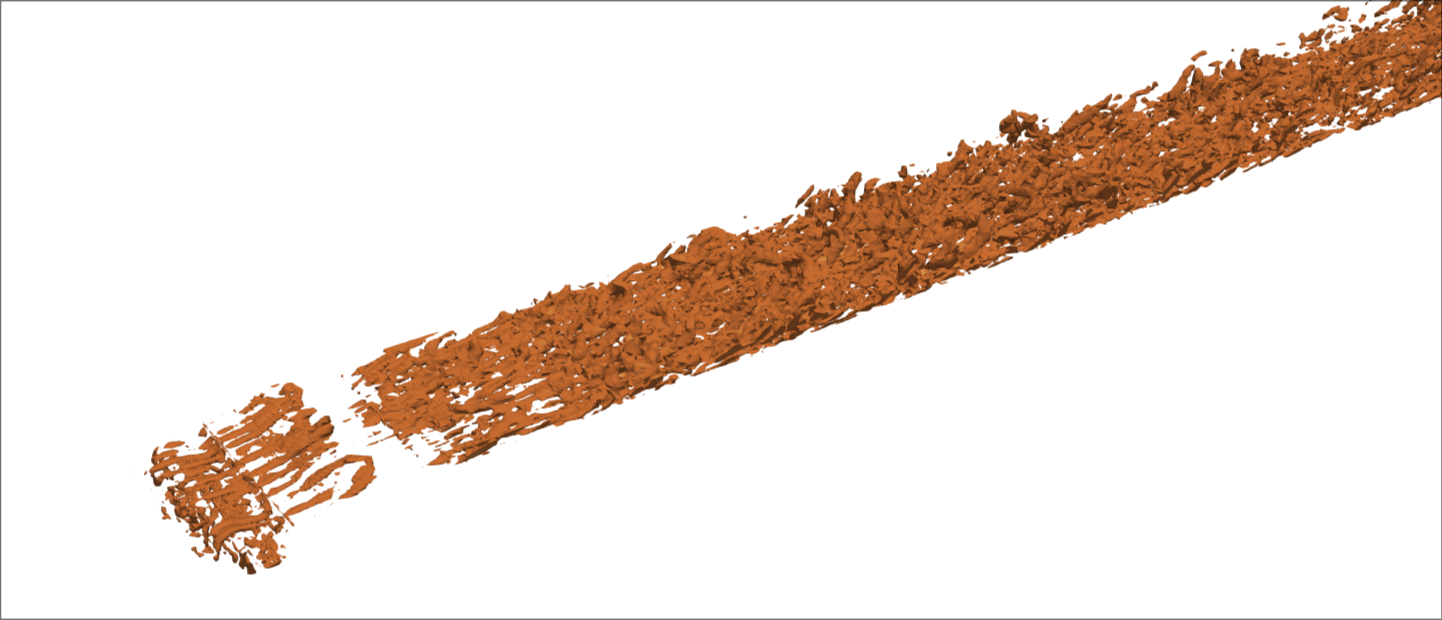
\includegraphics[width=\linewidth]{Images/d4_w19_transition3d.png}
  
\end{frame}
\begin{frame}
	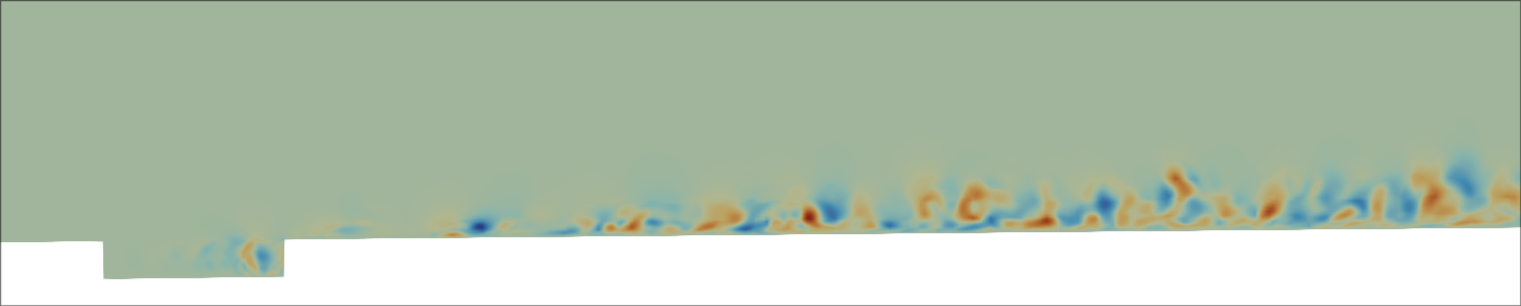
\includegraphics[width=\linewidth]{Images/d4_w19_transition2dslice.png}

	u, v, w, p spectrum (global stable mode frequency is dominant just after the gap)

	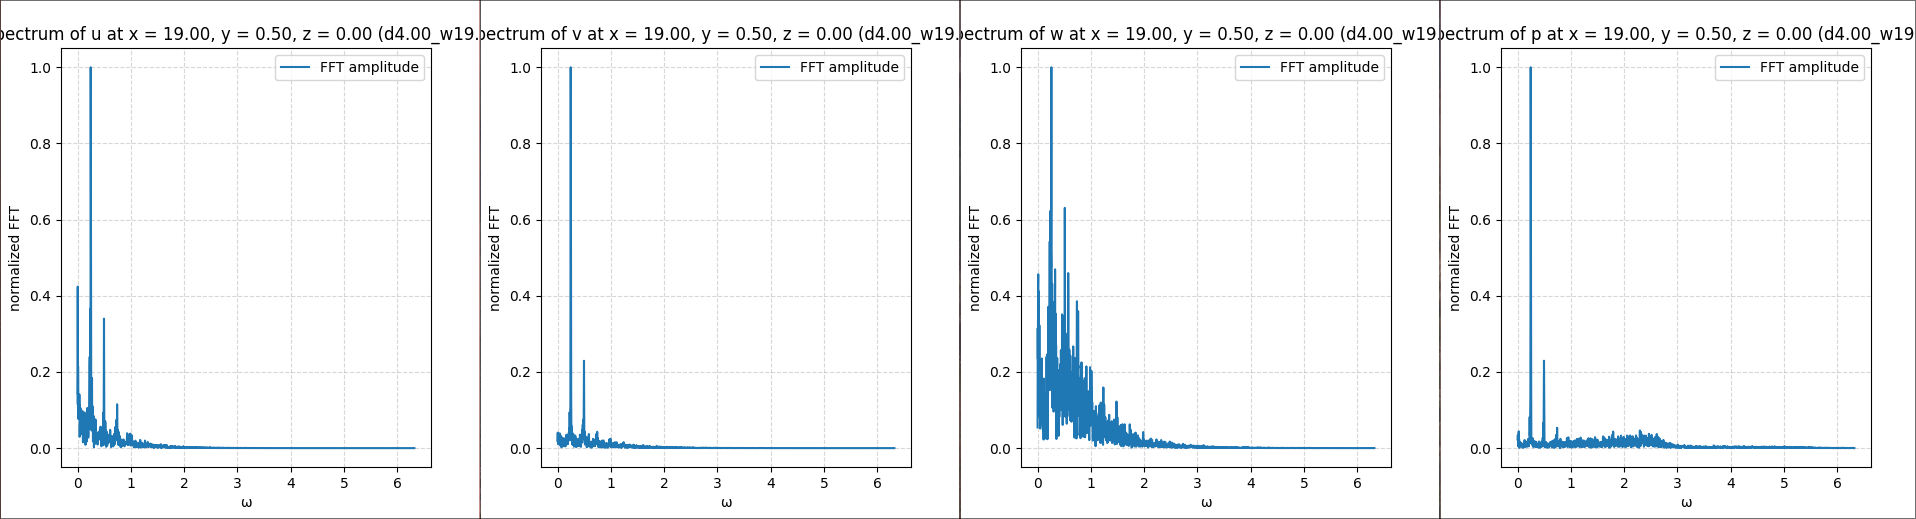
\includegraphics[width=\linewidth]{Images/d4_w19_fourierSpectrum.png}
\end{frame}

\begin{frame}
	\frametitle{Weakly unstable 2D mode, $d=4, w=18$ (=> 2d instability doesn't do anything)}
	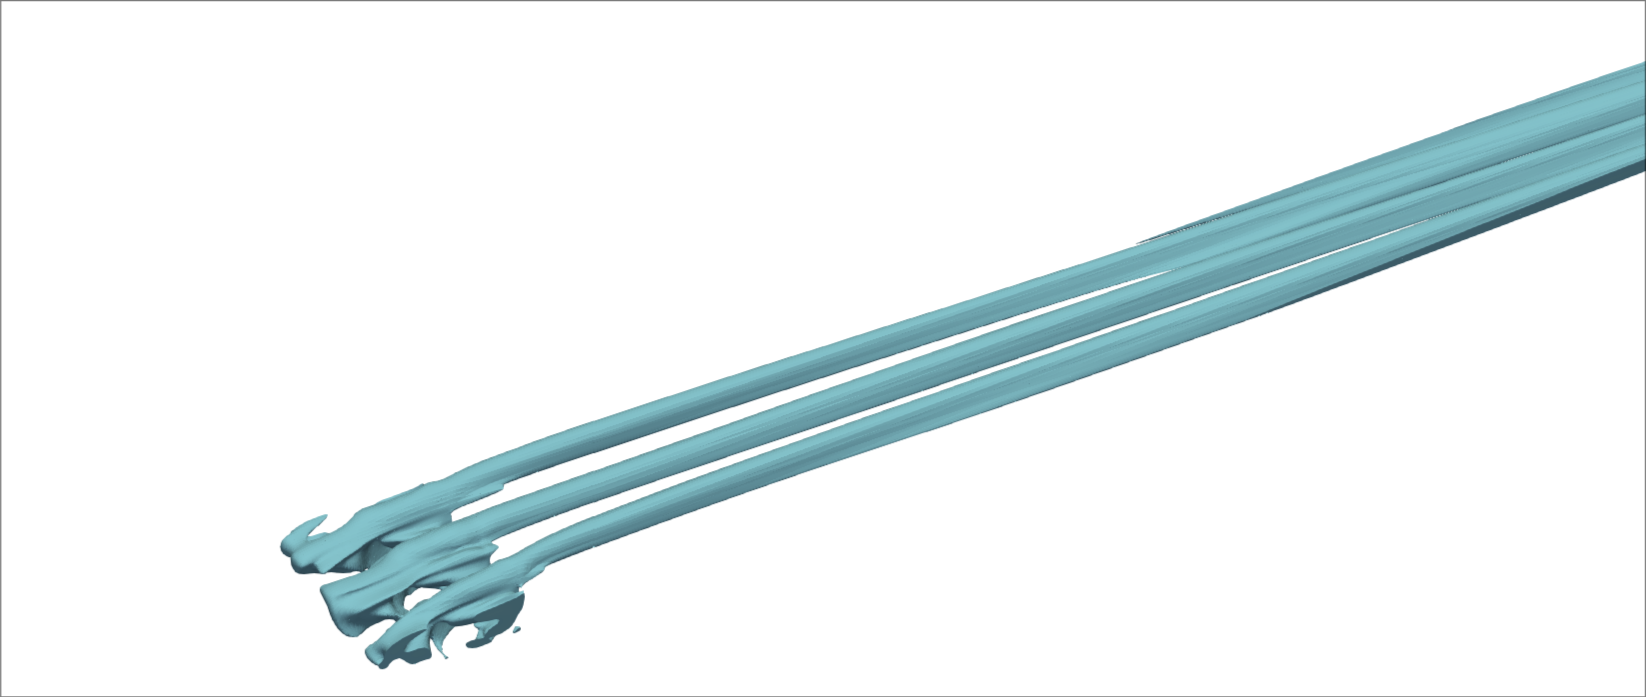
\includegraphics[width=\linewidth]{Images/d4_w18_weakUnstable2dmode.png}
\end{frame}

\end{document}
